\documentclass[10pt]{beamer}

\usepackage{custom}

\title{A Seriation Based Framework to Visualize Multiple Aspects of Road Transport from GPS Trajectories}
\date{International Conference on Intelligent Transportation, 2021}
\author{Alexandre Dubray \and Siegfried Nijssen \and Isabelle Thomas \and Pierre Schaus}
\institute{}
\titlegraphic{
    \includegraphics[scale=0.3]{../assets/aia-logo}
    \hfill
    \includegraphics[scale=0.3]{../assets/UCLouvain-logo}
}

\addbibresource{biblio.bib}

\begin{document}

\maketitle

\begin{frame}{An introducing example}
Imagine that we want to visualize the mean speed of the trucks, per municipality, for a given country.
\pause

First you compute the mean speed of the trucks in each municipality.
\pause

Then a color is assigned to each municipality, depending on this mean speed (from light to dark)
\pause

Finally, the municipalities are shown on a map with their color.
\pause

But how to extend that to handle multiple features at the same time?
\end{frame}

\begin{frame}{Existing solution}
    \begin{itemize}
        \item One graph/map per computed feature
        \item Cluster in some way the studied areas before showing them on a map
            \begin{itemize}
                \item Community detection, Self-Organizing Maps, ...
                \item Hard to analyze the features
            \end{itemize}
        \item In this work we propose a visualization that gives at one glance the geographical structure as well as feature interpretation
    \end{itemize}
\end{frame}

\begin{frame}{Overview of the framework}
\begin{figure}
    \centering
    \includegraphics[scale=0.45]{process.pdf}
\end{figure}

\pause

Two main questions
\begin{enumerate}
    \item How to order the spatial units?
    \item How to choose their color?
\end{enumerate}
\end{frame}

\begin{frame}{Ordering the units: Seriation}

    The goal of a seriation algorithm is to find a linear order of some objects so that similar objects are near each other.
    As an example, let us assume that we want to order these polygons.

    \begin{figure}
        \centering
        \includegraphics{figures/seriation-objects.pdf}
    \end{figure}

    The dissimilarity between two polygons is the difference between the number of edges they have.
\end{frame}

\begin{frame}{Ordering the units: Seriation}
    A possible ordering is the following

    \begin{figure}
        \centering
        \includegraphics{figures/seriation-order-1.pdf}
    \end{figure}

    The score of the ordering is computed as the sum of the successive dissimilarity.
    This ordering has a score of $2 + 2 + 1 + 2 = 7$
\end{frame}

\begin{frame}{Ordering the units: Seriation}
    The goal of a seriation algorithm is to find an ordering that minimize this score. In our example, the optimal ordering is the following
    \begin{figure}
        \centering
        \includegraphics{figures/seriation-order-2.pdf}
    \end{figure}
    with a score of $4$.
\end{frame}

\begin{frame}{Ordering the units: Seriation}
    In general
    \begin{itemize}
        \item The BSUs have more than one feature.
        \item The dissimilarity function depends on the type of the features.
        \item Multiple methods exist to solve the seriation problem. In this work we consider two of the most popular
            \begin{enumerate}
                \item Optimal-Leaf-Ordering \footfullcite{bar2001fast}
                \item Modelization as a Travelling Salesman Problem \footfullcite{laporte1978seriation}
            \end{enumerate}
    \end{itemize}

\end{frame}

\begin{frame}{The colors}

    A linear color scale is created using $n$ different colors evenly spaced.
    For instance, with four colors: blue; green; orange  and red, the following color scale is obtained.

    \begin{figure}
        \centering
        \includegraphics{figures/colorscale.pdf}
    \end{figure}

    \begin{itemize}
        \item Each of the $n$ colors has a value between $0$ (the first) and $1$ (the last) at regular intervals. In the above color scale, the green is at $0.33$ and orange at $0.66$.
        \item The intermediate colors are linearly interpolated
    \end{itemize}
\end{frame}

\begin{frame}{The colors}

    To assign a color to the BSUs, first their cumulative score (w.r.t the ordering) is computed why is then divided by the total score of the ordering.

    \begin{figure}
        \centering
        \includegraphics[scale=0.6]{figures/cumulative-score.pdf}
    \end{figure}
\end{frame}


\begin{frame}{The colors}

    \begin{itemize}
        \item If two BSUs have similar color, they have close features.
        \pause
        \item Seriation only provides "local" guarantees, thus a multicolor scale is needed
        \pause
        \item Some colors of the scale might be unassigned in case of big gaps between the BSUs.
    \end{itemize}
\end{frame}

\begin{frame}{The heatmap}
    \begin{figure}
        \centering
        \includegraphics[scale=0.7]{figures/heatmaps.pdf}
    \end{figure}
\end{frame}

\section{Results}

\begin{frame}{The data set}
    \begin{itemize}
        \item Trajectories of heavy good vehicles
        \item 1 day of data of all trucks that were on the Belgian territory
        \item Roughly $90,000$ vehicles and $30$ millions GPS ping
        \item BSU are 5 km by 5 km grid cells provided by Eurostat
        \item Features computed for each cell is the proportions of time passed in the following states: Driving; Resting; Work-related actions; In congestion.
    \end{itemize}
\end{frame}

\begin{frame}{Final visualization}
    \begin{figure}
        \centering
        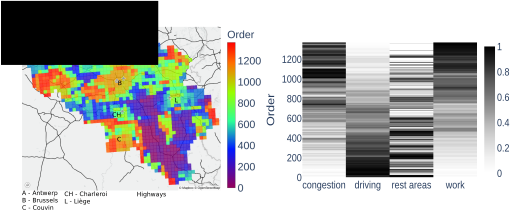
\includegraphics[scale=0.22]{figures/final-result.pdf}
    \end{figure}

    What can we infer on the geography of Belgium from this visualization ?
\end{frame}

\begin{frame}{Final visualization}
    \begin{figure}
        \centering
        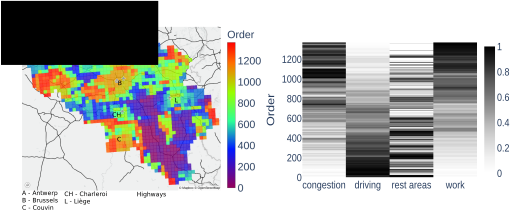
\includegraphics[scale=0.22]{figures/final-result.pdf}
    \end{figure}
    Three zones that match the structure of the country
    \begin{enumerate}
        \item Purple and blue : mainly driving
        \item Orange-red: Proportion of work and congestion much higher
        \item Green-yellow: in between
    \end{enumerate}
\end{frame}

\begin{frame}{Comparison}

    Comparison of our method and Self-Organizing Maps
    \begin{itemize}
        \item Overall the same structure
        \item Some areas are, however, less distinguishable
        \item No interpretation of the clusters in terms of features
    \end{itemize}
    \begin{figure}
        \centering
        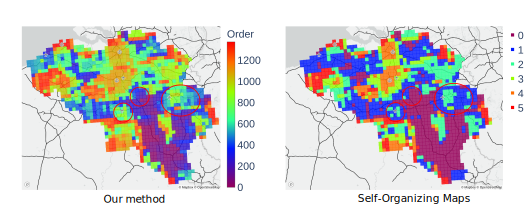
\includegraphics[scale=0.22]{figures/comparison.pdf}
    \end{figure}

\end{frame}

\begin{frame}{Conclusion \& Future work}
    The propose framework allows to quickly see
    \begin{itemize}
        \item The geographical structure given the features
        \item How this structure translates in term of features
    \end{itemize}
    \pause

    In the future, we could
    \begin{itemize}
        \item Integrate geographical informations in the seriation process
        \item Add time elements in the visualization
    \end{itemize}

\end{frame}

\end{document}

